% Compile with: xelatex -> biber -> xelatex -> xelatex
% !TeX program = xelatex
% !BIB program = biber


% 开启盲审格式 blindPeerReview=true (如:[type=bachelor,blindPeerReview=true])
\documentclass[type=bachelor,blindPeerReview=true]{bithesis}

% 此处仅列出常用的配置。全部配置用法请见「bithesis.pdf」手册。
\BITSetup{
  cover = {
    % 在封面中载入有「北京理工大学」字样的图片,如无必要请勿改动。
    headerImage = images/header.png,
    % 在封面标题中使用思源黑体,使用此选项可以保证与 Word 封面标题的字体一致。
    xiheiFont = STXIHEI.TTF,
    %% 使用以下参数来自定义封面日期
    % date = 2022年6月,
    % 本科生盲审要求删去封面,而不是隐藏封面信息。
    hideCoverInPeerReview = true,
  },
  info = {
    % 想要让某项封面信息留空(但是保留下划线),请传入空白符组成的字符串,如"{~}"。
    % 如需要换行,则用 “\\” 符号分割。
    title = 每周工作总结,
    author = nuclearslippers,
    keywords = {状态估计,KALMAN,Transformer},
  },
  style = {
    % 开启 Windows 平台下的中易宋体伪粗体。
    % windowsSimSunFakeBold = true,
    head = ,
  }
}

\usepackage{listings}
\usepackage{float}
\usepackage{xcolor} % 适用颜色框
\usepackage{tcolorbox}
\usepackage{bm}
\usepackage{amsmath}

% 大部分关于参考文献样式的修改,都可以通过此处的选项进行配置。
% 详情请搜索「biblatex-gb7714-2015 文档」进行阅读。
\usepackage[
  backend=biber,
  style=gb7714-2015,
  gbalign=gb7714-2015,
  gbnamefmt=lowercase,
  gbpub=false,
  doi=false,
  url=false,
  eprint=false,
  isbn=false,
]{biblatex}

% 参考文献引用文件位于 misc/ref.bib
\addbibresource{misc/ref.bib}


% 文档开始
\begin{document}

% 标题页面
% \input{misc/0_cover.tex}
\MakeCover


% ====== 原创性声明(PDF 格式)======
\begin{blindPeerReview}
  
\includepdf{misc/1_originality.pdf}\newpage
\end{blindPeerReview}
% ====== 原创性声明(LaTeX 格式)======
% %%
% The BIThesis Template for Bachelor Graduation Thesis
%
% 北京理工大学毕业设计(论文)原创性声明模板 —— 使用 XeLaTeX 编译
%
% Copyright 2020-2023 BITNP
%
% This work may be distributed and/or modified under the
% conditions of the LaTeX Project Public License, either version 1.3
% of this license or (at your option) any later version.
% The latest version of this license is in
%   http://www.latex-project.org/lppl.txt
% and version 1.3 or later is part of all distributions of LaTeX
% version 2005/12/01 or later.
%
% This work has the LPPL maintenance status `maintained'.
%
% The Current Maintainer of this work is Feng Kaiyu.
%
% Compile with: xelatex -> biber -> xelatex -> xelatex
%
% 如无特殊需要,本页面无需更改

\MakeOriginality


% 前置页面定义
\frontmatter

% 摘要
%\input{chapters/0_abstract.tex}

% 目录
%\MakeTOC

% 正文开始
\mainmatter

\chapter{问题描述}
\section{多目标检测与追踪问题描述}

给定图像序列${I_1, I_2,..., I_t}$, 每帧图像中有$M_t$个目标,其中t是当前帧号,每个目标的状态为$ s_1(t) $,其中状态一般包括位置,速度,加速度,朝向等。
\begin{equation}
	s_i(t) = \{ x,y,z,h,w,l,v_x,v_y,v_z,\theta \}
\end{equation}

当前帧的所有目标的状态就能表示成
\begin{equation}
	S(t) = \{ s_1(t), s_2(t),s_3(t),...,s_{M_t}(t) \}
\end{equation}

而每个目标的的轨迹则可以描述成
\begin{equation}
	s_i(1:t) = \{ s_i(1),s_i(2),s_i(3),...,s_i(t) \}
\end{equation}

则所有目标的状态集合就能表示成
\begin{equation}
	S(1:t) = \{ S_1. S_2,...S_t \}
\end{equation}

同理,我们类似的得到观测结果的定义,记作$ o_i(t),o_i(1:t),O(1:t) $。

而多目标跟踪任务就是通过观测结果找出所有目标的状态,我们用后验估计来进行描述。
\begin{equation}
	S(1:t) = argmax_{S(1:t)}P(S(1:t)|O(1:t))
\end{equation}

\section{问题的求解}
多目标检测与追踪一般的求解都基于TBD架构,如图\ref{dbt}所示。
\begin{figure}[H]
	\centering
	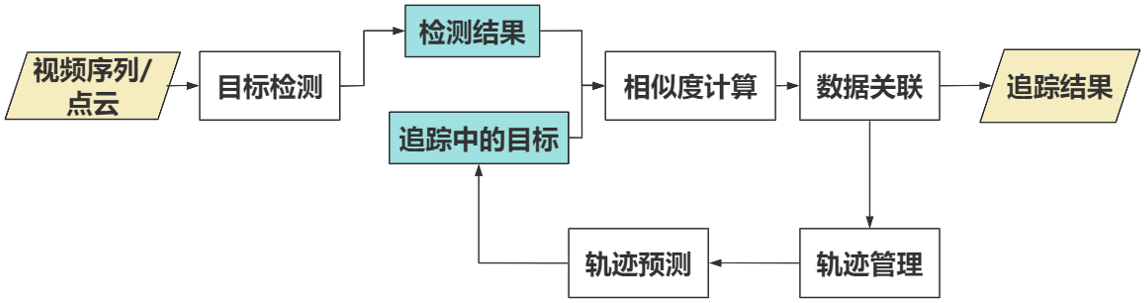
\includegraphics[width=\textwidth]{images/DBT.png}
	\caption{基于检测的追踪框架}
	\label{dbt}
\end{figure}


\section{滤波的作用}
主要概括,滤波的作用主要包括两个部分,融合多个传感器的追踪结果以及对目标进行预测,最终的目的都是为了得到更好的估计值。
它主要应用在图\ref{dbt}中轨迹预测部分。

\begin{tcolorbox}[]
	首先构建线性系统的状态空间描述:
	$$ \mathbf{x}_{t} = \mathbf{A} \mathbf{x}_{t-1} + \mathbf{B} \mathbf{u}_{t} + \bm{\epsilon}_{t} $$
	$$  \mathbf{z}_{t} = \mathbf{H} \mathbf{x}_{t} + \bm{\delta}_{t} $$
	
	接着利用卡尔曼滤波器进行最优状态估计:
	\begin{equation}
		\hat{\bm{x}}_{t}^{-} =  \bm{A} \hat{\bm{x}}_{t} + \bm{B} \bm{u}_t
	\end{equation}
	\begin{equation}
		\bm{\Sigma}_{t}^{-} = \bm{A} \bm{P}_{t-1} \bm{A}^{T} + \bm{Q}
	\end{equation}
	\begin{equation}
		\bm{K}_t = \frac{\bm{\Sigma}_{t}^{-} \bm{H}^{T}}{\bm{H} \bm{P}_{t}^{-} \bm{H}^{T} + \bm{R} }
	\end{equation}
	\begin{equation}
		\hat{\bm{x}}_t = \hat{\bm{x}}_{t-1} + \bm{K}_t(\bm{z}_t - \bm{H} \hat{\bm{x}}^{-})
	\end{equation}
	\begin{equation}
		\bm{P}_t = (\bm{I} - \bm{K}_t \bm{H}) \bm{P}_{t}^{-}
	\end{equation}
	
\end{tcolorbox}

\section{发展和思考}
1. \textbf{发展}

想要提高追踪的效果(精度,速度),可以从多个角度进行提高。大致可以包括几个方面:

仍旧基于BDT框架:追踪器的提升,数据融合方法的提升,数据关联的提升,滤波器的提升(包括模型改进)。

新的框架:端到端\cite{10610979},基于点的移动的追踪\cite{wu2024moving}。

2. \textbf{思考}

首先确定融合的框架:DBT和神经网络融合结构。
接着确定数据关联方式,倾向于用特征值(点)
然后改进滤波器的结构:模型的改进(长时间拟合),噪声的优化(A-KIT)
最后,连接最新的检测器。

实际实验:标定,ROS表示

\section{工作总结}
时间:11.18-11.24

工作内容:
对研究问题进行了数学上的描述;
学习了DFR-FastMOT和ByteTrack两篇文章,它们均对遮挡情况提出了不同解决方法;

工作展望:
将BYTE的思想移植到之前的追踪器中,看看提升的效果。

\chapter{DFR-FastMOT: Detection Failure Resistant Tracker for Fast  Multi-Object Tracking Based on Sensor Fusion(ICRA2023)\cite{10160328}}

\section{解决问题}
文章主要针对目标追踪中的遮挡问题做了许多工作。
非学习算法往往只保存一小段的轨迹,因此难以应对长时间的遮挡情况。
文章设计了一种代数的数据关联公式从而降低了需要计算复杂度,从而可以处理更长时间的轨迹。

\section{解决算法}
\begin{figure}[htbp]
	\centering
	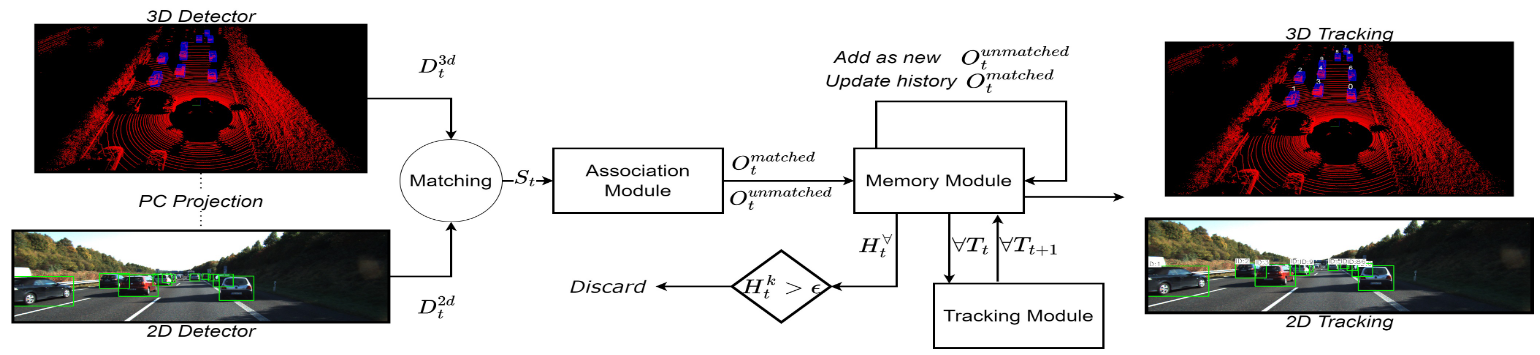
\includegraphics[width=\textwidth]{images/DFRMOT/framework.png}
	\caption{整体框架}
	\label{framework}
\end{figure}

\subsection{关联矩阵的引入}
为了提高计算的效率,文章为每种传感器设计了一个关联矩阵,矩阵的每个元素代表前一时刻对象(轨迹)的估计值和当前时刻检测值的关联程度。

\begin{figure}[H]
	\centering
	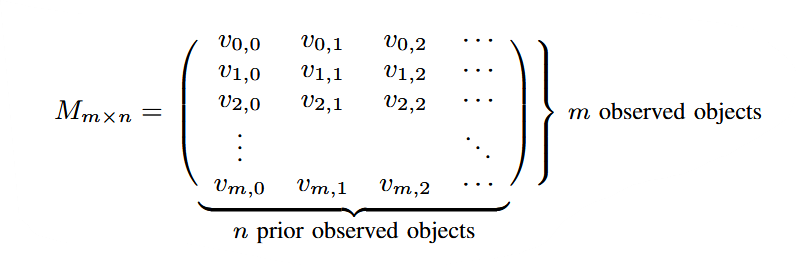
\includegraphics[width=0.8\textwidth]{images/DFRMOT/matrix.png}
\end{figure}

\begin{tcolorbox}[]

\hspace{22pt}$v_{i,j}$代表关联值,公式\ref{equ_0}处理2D情况,记作$M_c$。公式\ref{equ_1}处理3D情况,记作$M_l$。公式\ref{equ_2}将两种情况进行统一,记作$M_f$。

\begin{equation}\label{equ_0}
	v_{ij} = 
	\begin{cases}
		v_{IoU}&:v_{IoU}\leq a_c\\
		0&:\text{Otherwise}.
	\end{cases}
\end{equation}

\begin{equation}\label{equ_1}
	v_{ij} = 
	\begin{cases}
		v_{dist} & :v_{dist} < a_l\\
		a_l & :\text{Otherwise}.
	\end{cases}
\end{equation}

\begin{equation} \label{equ_2}
\begin{cases}
	M_f &= \alpha_c M_c + \alpha (1 - M_t), \\
	\alpha_c + \alpha_l &= 1, \\
	\alpha_c , \alpha_l &\leq 1.
\end{cases}
\end{equation}

\hspace{22pt}得到所有关联矩阵之后,便可以进行数据关联。文章采用了类匈牙利算法来实现该步骤。
最后所有的计算复杂度为:
$$ \mathcal{O}(2mn) \rightarrow \mathcal{O}(m^2n^2) \rightarrow \mathcal{O}(m^2n^2) $$

\end{tcolorbox}

\subsection{其它处理方法}
1. 3D距离函数的选用

为了处理遮挡的情况,文章采用了3D中心距离来衡量两个目标的相似程度,而不是传统的IoU。当出现长时间的遮挡情况时,去计算IoU是十分困难的,而计算3D的距离则更容易实现。

2. KF计算简化

在用KF计算目标下一时刻的状态时,需要进行大量的矩阵运算。为此,作者采用最少点数来描述目标位置:2D两个,3D两个。

\section{文章结果}
文章通过使用不同质量的检测器来模拟遮挡的效果。结果表明,文章显著提高了低质量检测器的追踪效果。整体而言,追踪的精度也有所提高。
\begin{figure}
	\centering
	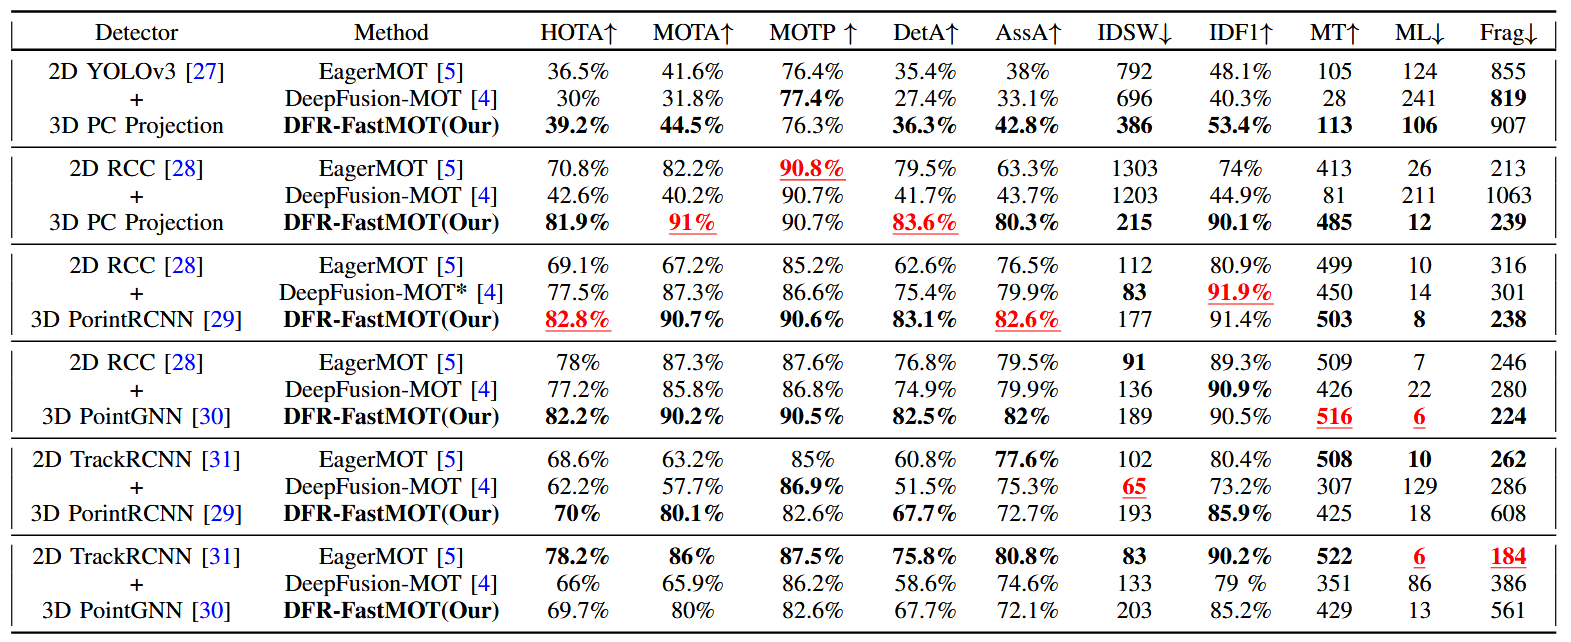
\includegraphics[width=\textwidth]{images/DFRMOT/result.png}
\end{figure}


\section{学习总结}
DFRMOT也是采用DBT追踪框架,具体内容也基本和EagerMOT相似。其主要工作在于提出了一种提高计算效率的关联矩阵,由此多出的冗余可以用来计算更长时间的目标,间接的提高了应对遮挡的能力。

所以,在自己设计的追踪器上,就可以采用本文设计的关联矩阵提高计算效率。
此外,本外还在细节上提出了许多加速方法,我们可以直接应用他的计算框架来完成更复杂的任务。


\chapter{"ByteTrack: Multi-Object Tracking by Associating Every Detection Box(ECCV2022)"\cite{zhang2022bytetrack}}

数据关联问题是MOT的核心,本文就此提出了一种新的关联方法,显著提高了追踪效果。
数据关联问题可以转化成一个最优化问题:

\begin{tcolorbox}
	
	\begin{equation}
		\min_{\mathbf{A}} \sum_{i=1}^{N_t} \sum_{j=1}^{M_t} \mathcal{C}(d_{t,i}, t_{t,j}) \cdot A_{i,j}
	\end{equation}
	
	\hspace{22pt}其中,\(\mathbf{A}\) 是一个 \(N_t \times M_t\) 的关联矩阵,\(A_{i,j}\) 表示检测目标 \(d_{t,i}\) 与轨迹 \(t_{t,j}\) 的关联状态,定义为:
	\[
	A_{i,j} = \begin{cases} 
		1, & \text{如果检测目标 } d_{t,i} \text{ 与轨迹 } t_{t,j} \text{ 关联} \\
		0, & \text{否则}
	\end{cases}
	\]
	
	\hspace{22pt}\textbf{约束条件:}
	
	\begin{itemize}
		\item 每个检测目标最多关联一个轨迹:
		\[
		\sum_{j=1}^{M_t} A_{i,j} \leq 1, \quad \forall i \in \{1, 2, \ldots, N_t\}
		\]
		\item 每个轨迹最多关联一个检测目标:
		\[
		\sum_{i=1}^{N_t} A_{i,j} \leq 1, \quad \forall j \in \{1, 2, \ldots, M_t\}
		\]
	\end{itemize}
	
	\hspace{22pt}\textbf{关联成本函数:}
	关联成本函数 \(\mathcal{C}(d_{t,i}, t_{t,j})\) 通常基于检测目标与轨迹之间的相似性度量,例如:
	
	\[
	\mathcal{C}(d_{t,i}, t_{t,j}) = -\text{similarity}(\mathbf{x}_{t,i}, \mathbf{y}_{t,j})
	\]
	
	其中,\(\text{similarity}(\mathbf{x}_{t,i}, \mathbf{y}_{t,j})\) 是一个相似性函数,可以基于位置、外观特征、运动状态等计算。
	
\end{tcolorbox}

\section{文章算法}

文章的想法大致可以总结为:关联所有检测框。对于高置信度的检测结果,采用运动学和外貌特征的相似度计算。对于低置信度的检测结果,只采用运动学的相似度计算。

这是因为低置信度的检测结果往往代表着被遮挡,故BTYE追踪器对遮挡物体有着较好的应对效果。

\begin{tcolorbox}
	\hspace{22pt}\textbf{关联成本函数1:}
	\begin{equation}
		\mathcal{C}_1(d_{t,i}, t_{t,j}) = \text{IOU}(\mathbf{B}_{t,i}, \hat{\mathbf{B}}_{t,j}) + \lambda \cdot \text{Re-ID}(d_{t,i}, t_{t,j})
	\end{equation}
	
	\begin{itemize}
		\item \( \mathbf{B}_{t,i} \):第 \( t \) 帧中第 \( i \) 个检测结果的边界框。
		\item \( \hat{\mathbf{B}}_{t,j} \):第 \( t \) 帧中第 \( j \) 个轨迹的Kalman估计边界框。
		\item \( \text{IOU}(\mathbf{B}_{t,i}, \hat{\mathbf{B}}_{t,j}) \):边界框 \( \mathbf{B}_{t,i} \) 和 \( \hat{\mathbf{B}}_{t,j} \) 的交并比。
		\item \( \text{Re-ID}(d_{t,i}, t_{t,j}) \):检测目标 \( d_{t,i} \) 和轨迹 \( t_{t,j} \) 的Re-ID相似度。
	\end{itemize}
	
	其中,\( \lambda \) 是一个权重参数,用于平衡IOU和Re-ID相似度在成本函数中的相对重要性。
	
	\hspace{22pt}\textbf{关联成本函数2:}
	\begin{equation}
		\mathcal{C}_2(d_{t,i}, t_{t,j}) = \text{IOU}(\mathbf{B}_{t,i}, \hat{\mathbf{B}}_{t,j})
	\end{equation}
	
\end{tcolorbox}

\section{实验结果}
文章也是采用的DBT框架,检测器用的当时最先进的YOLOX,数据关联用的本文提出的方法,两者相结合即BTYE追踪器。其在MOT17数据集上的结果如图\ref{byte_1}所示。

\begin{figure}[H]
	\centering
	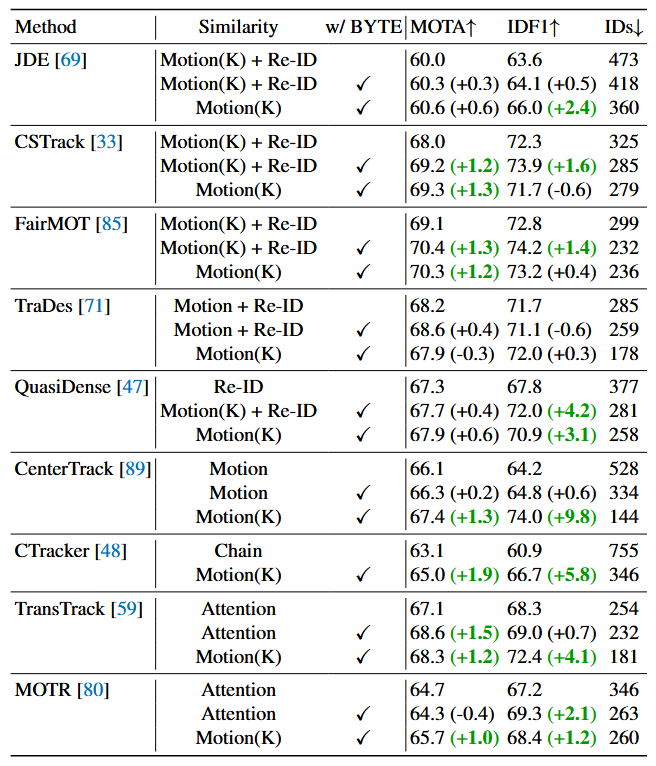
\includegraphics[width=0.8\textwidth]{images/BYTE/result1.png}
	\caption{在MOT17数据集上的结果}
	\label{btye_1}
\end{figure}


\section{论文学习}
数据关联的方法还有许多,本文的方法是基于SORT(DEEPSORT)的方法衍生而来,更偏向工程应用的一种方法。
数学上还有很多方法,例如最近邻、航迹分裂、01整数规则、联合概率数据关联(JPDA)和神经网络。



% 后置部分
\backmatter



% 结论
%
\begin{conclusion}
  本文结论……
\end{conclusion}



% 参考文献
\begin{bibprint}
\printbibliography[heading=none]
\end{bibprint}



\end{document}
